\documentclass{beamer}
\usepackage[utf8]{inputenc}
\usepackage[T1]{fontenc}
\usepackage[french]{babel}
\usepackage{graphicx}
\usepackage{amsmath}
\usepackage{listings}
\usepackage{xcolor}
\usepackage{booktabs}
\usepackage{tikz}
\usetikzlibrary{shapes.geometric, arrows.meta, positioning, fit}
\usepackage{hyperref}

\usetheme{Madrid}
\usecolortheme{default}

\definecolor{bleuPigier}{RGB}{0, 70, 127}
\setbeamercolor{structure}{fg=bleuPigier}

\setbeamertemplate{headline}{
  \leavevmode
  \begin{beamercolorbox}[wd=\paperwidth,ht=2.8ex,dp=1ex,right,rightskip=0.5cm]{structure}
    \tiny\color{white}
    Code source disponible sur GitHub :
    \href{https://github.com/Arnel7/projet-Infrastructure-Big-data}{https://github.com/Arnel7/projet-Infrastructure-Big-data}
    \hspace{0.3cm}
  \end{beamercolorbox}
}

\title[Projet Big Data]{Infrastructure Big Data}
\subtitle{Projet d'examen --- Deux analyses de données}
\author{LAWSON Arnel}
\date{28 Février 2026}

\setbeamertemplate{footline}{
  \leavevmode
  \hbox{
    \begin{beamercolorbox}[wd=.5\paperwidth,ht=2.5ex,dp=1.5ex,leftskip=.3cm]{author in head/foot}
      \usebeamerfont{author in head/foot}\insertshortauthor
    \end{beamercolorbox}
    \begin{beamercolorbox}[wd=.35\paperwidth,ht=2.5ex,dp=1.5ex,center]{title in head/foot}
      \usebeamerfont{title in head/foot}\insertshorttitle
    \end{beamercolorbox}
    \begin{beamercolorbox}[wd=.15\paperwidth,ht=2.5ex,dp=1.5ex,right,rightskip=.3cm]{date in head/foot}
      \usebeamerfont{date in head/foot}\insertframenumber{}/\inserttotalframenumber
    \end{beamercolorbox}
  }
  \vskip0pt
}

\begin{document}

\begin{frame}
  \titlepage
\end{frame}

\begin{frame}{Sommaire}
  \tableofcontents
\end{frame}

% ==========================================
\section{Projet 1 : Enquête de marché}
% ==========================================

\begin{frame}{Projet 1 --- Contexte et données}
  \begin{block}{Contexte}
    Une entreprise souhaite lancer une activité de vente de plats jetables.
    Une enquête terrain a été réalisée pour comprendre les attentes des clients.
  \end{block}

  \begin{columns}
    \column{0.5\textwidth}
    \textbf{Données}
    \begin{itemize}
      \item Fichier : \texttt{enquête.xlsx}
      \item \textbf{123 répondants}
      \item \textbf{29 variables}
    \end{itemize}

    \column{0.5\textwidth}
    \textbf{Outils utilisés}
    \begin{itemize}
      \item Python 3.12
      \item pandas, matplotlib
      \item seaborn, numpy
    \end{itemize}
  \end{columns}
\end{frame}

\begin{frame}{Projet 1 --- Préparation des données}
  \begin{itemize}
    \item Renommage des 29 colonnes en noms courts
    \item Suppression de la colonne \texttt{photo\_url} (non pertinente)
    \item Conversion des montants textuels en numériques
      \begin{itemize}
        \item \texttt{"10.000f"} $\rightarrow$ \texttt{10000.0}
        \item \texttt{"5000 à 10000f"} $\rightarrow$ \texttt{7500.0} (milieu de plage)
        \item \texttt{"20 ou 35 milles"} $\rightarrow$ \texttt{27500.0}
      \end{itemize}
    \item Remplacement des NaN numériques par la \textbf{médiane}
    \item Harmonisation : fréquences, quantités, intention d'achat
    \item Résultat : \textbf{0 valeur manquante}, \textbf{28 colonnes}
  \end{itemize}
\end{frame}

\begin{frame}{Projet 1 --- Analyse exploratoire}
  \begin{columns}
    \column{0.5\textwidth}
    \textbf{Activités des répondants}
    \begin{itemize}
      \item Majoritairement restaurateurs
      \item Mets africains et européens
      \item Fast-foods et snacks
    \end{itemize}

    \vspace{0.3cm}
    \textbf{Utilisation actuelle}
    \begin{itemize}
      \item \textbf{100\%} utilisent des emballages jetables
      \item 48\% : 1--10 unités/jour
      \item 38\% : 10--30 unités/jour
      \item 14\% : 30--50 unités/jour
    \end{itemize}

    \column{0.5\textwidth}
    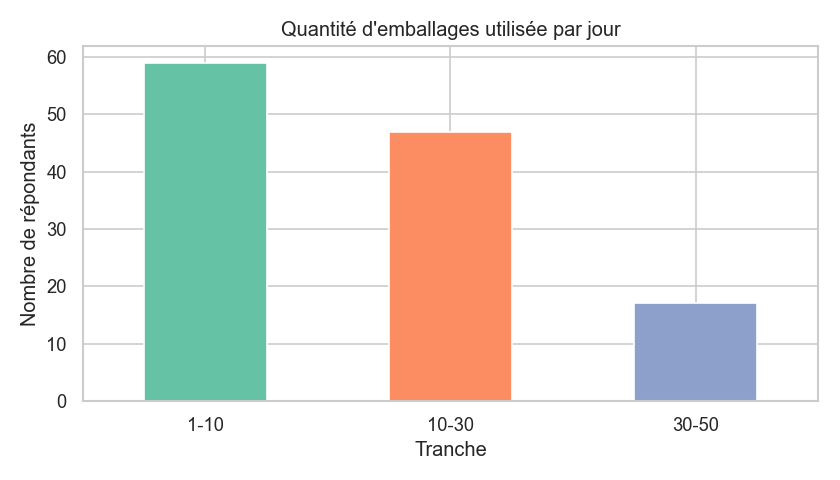
\includegraphics[width=\textwidth]{projet1/graphiques/03_quantite_par_jour.png}
  \end{columns}
\end{frame}

\begin{frame}{Projet 1 --- Préférences des clients}
  \begin{columns}
    \column{0.5\textwidth}
    \begin{itemize}
      \item \textbf{Compartiments} : combinaisons 1--3 compartiments les plus demandées
      \item \textbf{Contenance} : 850 ML préférée (1 compartiment)
      \item \textbf{Design} : 78.9\% veulent une fenêtre transparente
      \item \textbf{Matériau} : Carton et Bioplastiques en tête
    \end{itemize}

    \column{0.5\textwidth}
    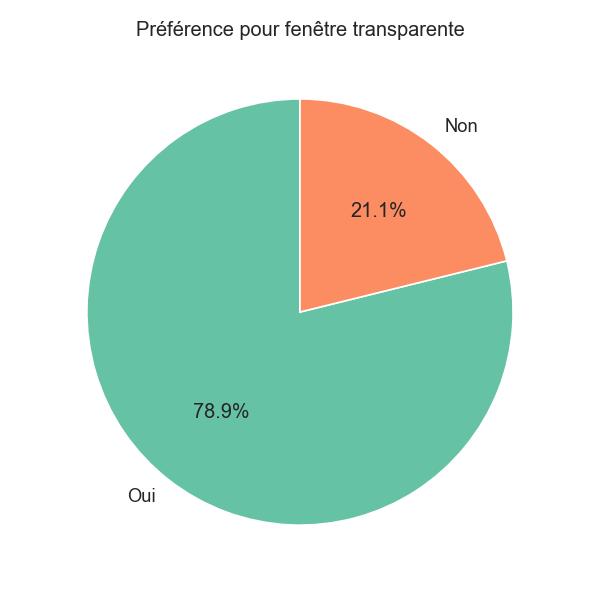
\includegraphics[width=\textwidth]{projet1/graphiques/06_fenetre_transparente.png}
  \end{columns}
\end{frame}

\begin{frame}{Projet 1 --- Sensibilité au prix}
  \begin{columns}
    \column{0.5\textwidth}
    \begin{block}{Chiffres clés}
      \begin{itemize}
        \item Prix médian actuel : \textbf{3 500 FCFA/centaine}
        \item Budget mensuel médian : \textbf{7 000 FCFA}
        \item 36.6\% prêts à payer plus cher
        \item 58.5\% répondent "peut-être"
      \end{itemize}
    \end{block}

    \column{0.5\textwidth}
    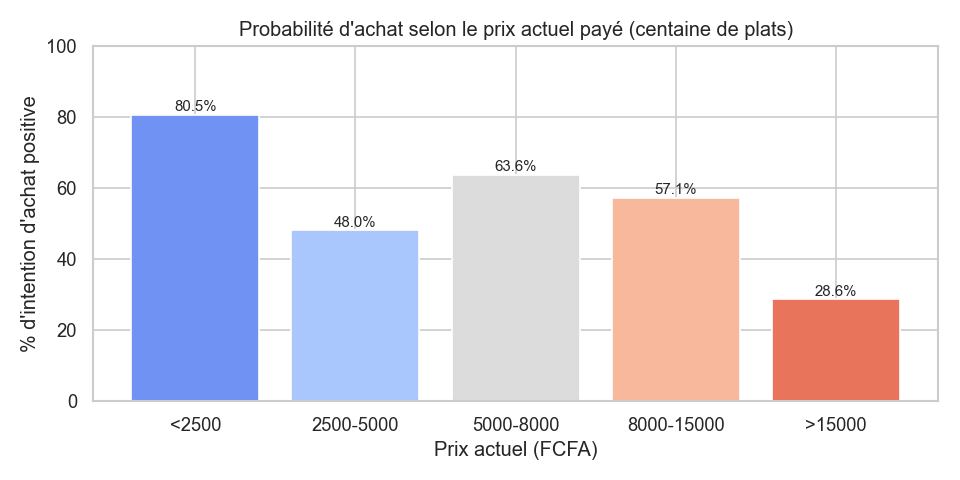
\includegraphics[width=\textwidth]{projet1/graphiques/18_prix_vs_intention_achat.png}
  \end{columns}
\end{frame}

\begin{frame}{Projet 1 --- Intention d'achat}
  \begin{columns}
    \column{0.5\textwidth}
    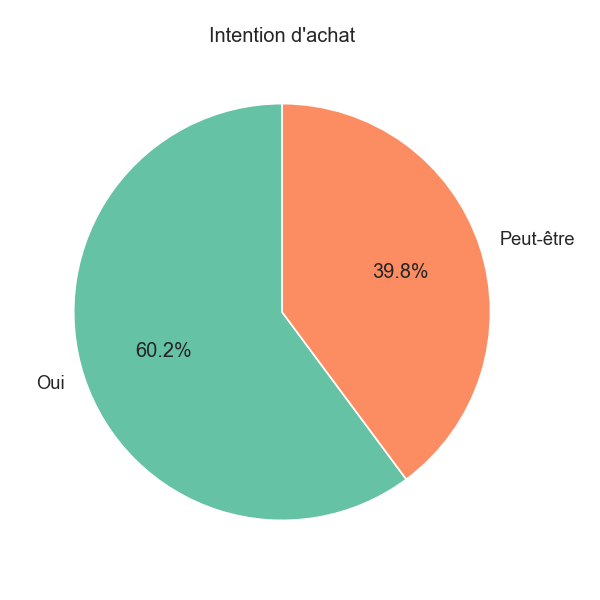
\includegraphics[width=\textwidth]{projet1/graphiques/12_intention_achat.png}

    \column{0.5\textwidth}
    \begin{itemize}
      \item \textbf{60.2\%} ont une intention d'achat positive
      \item Livraison \textbf{hebdomadaire} préférée
      \item \textbf{Distribution locale} plébiscitée
    \end{itemize}

    \vspace{0.3cm}
    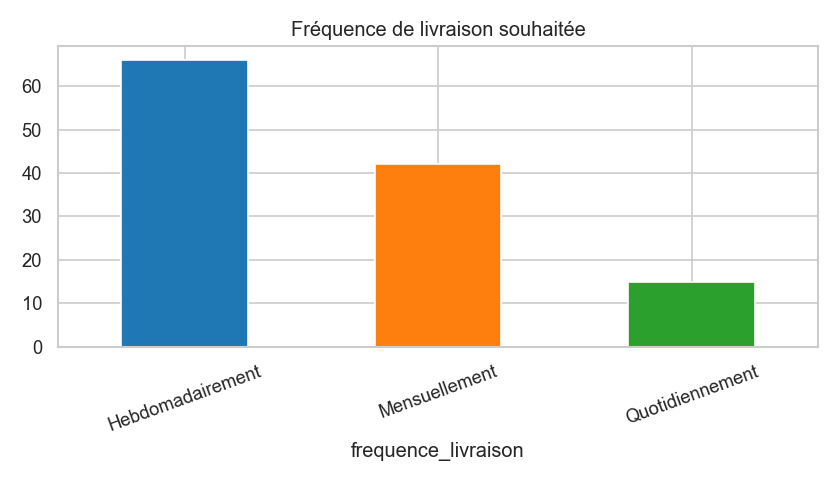
\includegraphics[width=\textwidth]{projet1/graphiques/13_frequence_livraison.png}
  \end{columns}
\end{frame}

\begin{frame}{Projet 1 --- Segmentation des clients}
  \begin{columns}
    \column{0.5\textwidth}
    \textbf{Méthode : règles métier}
    \begin{itemize}
      \item Score basé sur quantité, budget et disposition à payer plus
    \end{itemize}

    \vspace{0.2cm}
    \begin{tabular}{lcc}
      \toprule
      Segment & Nb & Budget moy. \\
      \midrule
      B - Moyen & 54 & 11 889 FCFA \\
      C - Petit & 69 & 5 152 FCFA \\
      \bottomrule
    \end{tabular}

    \column{0.5\textwidth}
    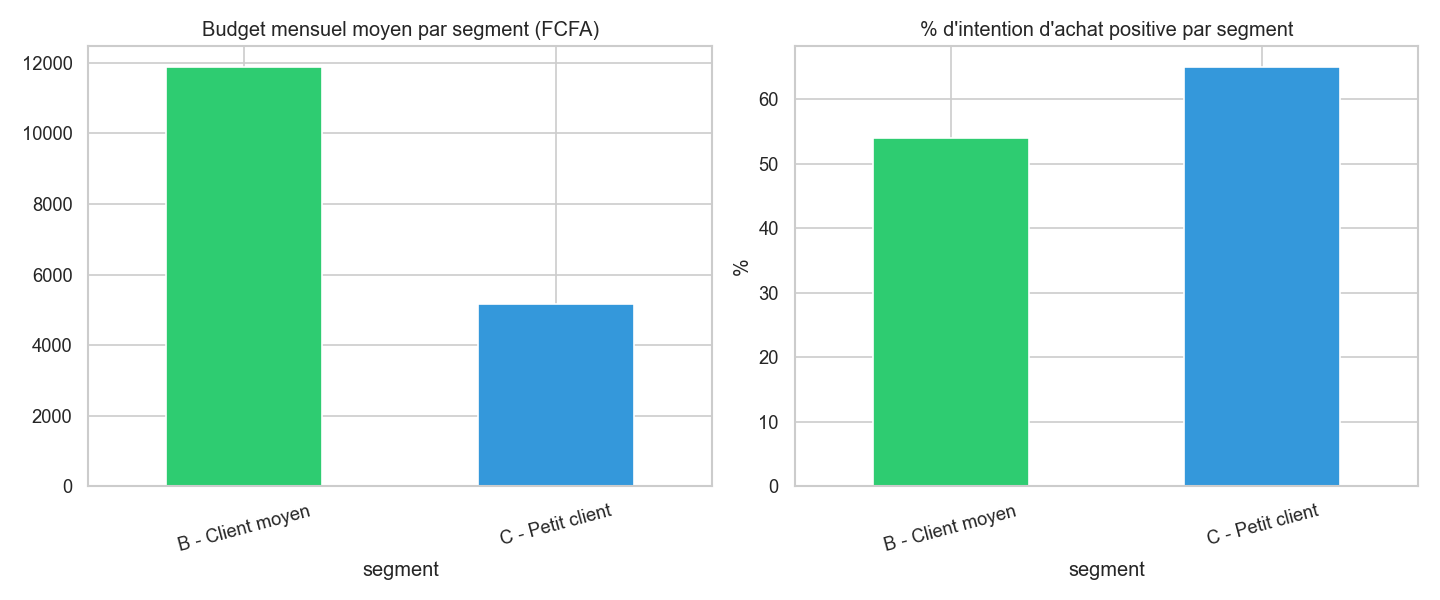
\includegraphics[width=\textwidth]{projet1/graphiques/17_profil_segments.png}
  \end{columns}
\end{frame}

\begin{frame}{Projet 1 --- Recommandations}
  \begin{block}{Produit}
    \begin{itemize}
      \item Multi-compartiments (1--3), carton ou bioplastique, avec fenêtre
      \item Contenance cible : 850 ML (1 comp.), 800 ML (2 comp.)
    \end{itemize}
  \end{block}

  \begin{block}{Politique de prix}
    \begin{itemize}
      \item Positionner entre \textbf{3 000 et 4 000 FCFA} la centaine
      \item Offrir une gamme premium pour les 36.6\% prêts à payer plus
    \end{itemize}
  \end{block}

  \begin{block}{Approvisionnement}
    \begin{itemize}
      \item Priorité à la \textbf{distribution locale}
      \item Cadence de livraison \textbf{hebdomadaire}
    \end{itemize}
  \end{block}
\end{frame}

% ==========================================
\section{Projet 2 : Analyse Big Data retail}
% ==========================================

\begin{frame}{Projet 2 --- Contexte et données}
  \begin{block}{Contexte}
    Analyse de données de ventes en commerce de détail avec \textbf{Apache Spark (PySpark)}.
    Traitement sur serveur distant Ubuntu 31 GB RAM.
  \end{block}

  \begin{columns}
    \column{0.5\textwidth}
    \textbf{Données}
    \begin{itemize}
      \item Fichier : \texttt{retailsale.csv}
      \item \textbf{109 443 lignes}
      \item \textbf{10 colonnes}
      \item 311 produits, 107 magasins
    \end{itemize}

    \column{0.5\textwidth}
    \textbf{Outils}
    \begin{itemize}
      \item PySpark 4.1.1
      \item Spark MLlib
      \item Python 3.13 (serveur)
      \item matplotlib, seaborn
    \end{itemize}
  \end{columns}
\end{frame}

\begin{frame}{Projet 2 --- Prétraitement avec Spark}
  \begin{itemize}
    \item Chargement CSV avec inférence de schéma automatique
    \item Suppression de \texttt{promo\_type\_2} (sans variabilité analytique)
    \item Remplacement des NaN de \texttt{promo\_bin\_1} (89\%) par \texttt{"Aucune"}
    \item Suppression de la ligne avec NaN dans price, stock, sales
    \item Conversion \texttt{date} $\rightarrow$ \texttt{DateType}
    \item Recast : sales (int), stock (int), price (float)
    \item Nouvelles variables créées :
      \begin{itemize}
        \item \texttt{revenu\_calcule} = sales $\times$ price
        \item \texttt{annee}, \texttt{mois}, \texttt{semaine}
        \item \texttt{en\_promotion} : binaire basé sur \texttt{promo\_bin\_1}
      \end{itemize}
    \item Résultat : \textbf{109 442 lignes}, \textbf{0 NaN}
  \end{itemize}
\end{frame}

\begin{frame}{Projet 2 --- Statistiques descriptives}
  \begin{tabular}{lcccc}
    \toprule
    Variable & Moyenne & Std & Min & Max \\
    \midrule
    sales & 0.46 & 2.22 & 0 & 161 \\
    revenu\_calcule & 1.57 & 7.39 & 0 & 796.95 \\
    stock & 16.01 & 40.79 & 0 & 2 892 \\
    price & 8.92 & 10.87 & 0.25 & 219.90 \\
    \bottomrule
  \end{tabular}

  \vspace{0.4cm}
  \begin{alertblock}{Observation clé}
    La médiane des ventes est \textbf{0} : la majorité des combinaisons
    produit-magasin-date n'enregistrent aucune vente.
    Ce phénomène est typique des données retail à grande dimension.
  \end{alertblock}
\end{frame}

\begin{frame}{Projet 2 --- Top produits et magasins}
  \begin{columns}
    \column{0.5\textwidth}
    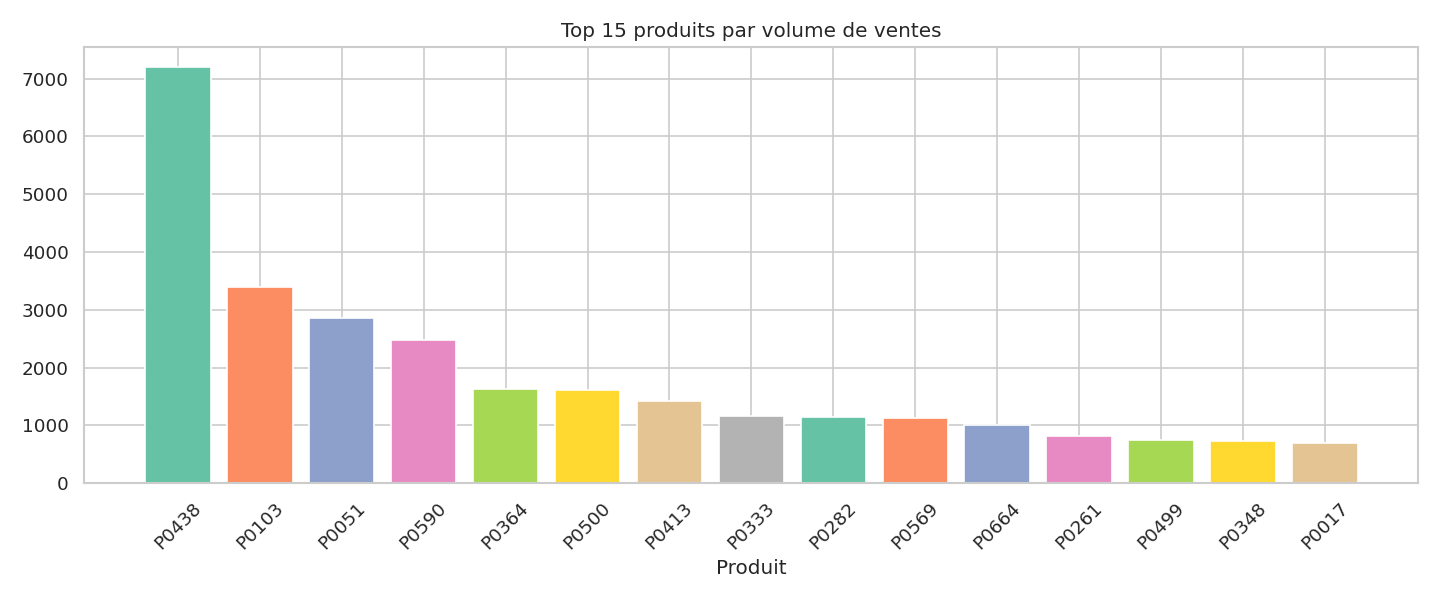
\includegraphics[width=\textwidth]{projet2/graphiques/01_ventes_par_produit.png}

    \column{0.5\textwidth}
    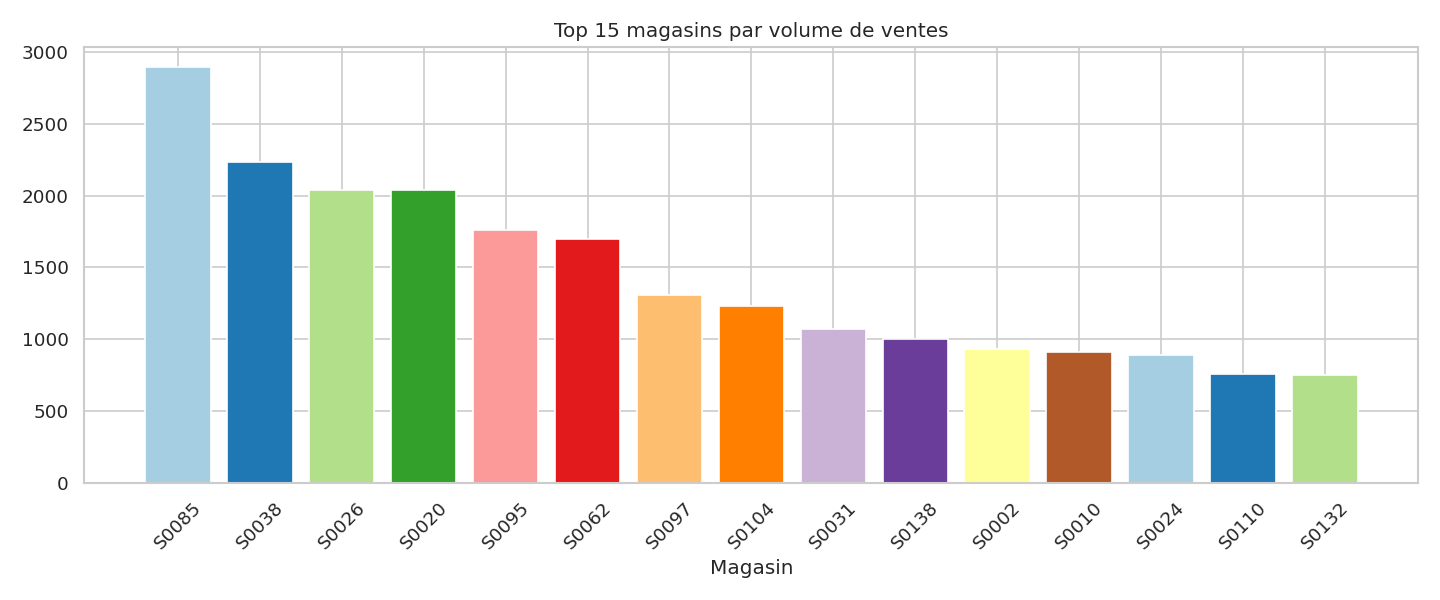
\includegraphics[width=\textwidth]{projet2/graphiques/03_ventes_par_magasin.png}
  \end{columns}

  \vspace{0.2cm}
  \begin{itemize}
    \item \textbf{P0438} est le produit le plus vendu (7 194 unités)
    \item \textbf{S0085} est le magasin le plus performant (2 893 unités)
  \end{itemize}
\end{frame}

\begin{frame}{Projet 2 --- Évolution temporelle}
  \begin{columns}
    \column{0.5\textwidth}
    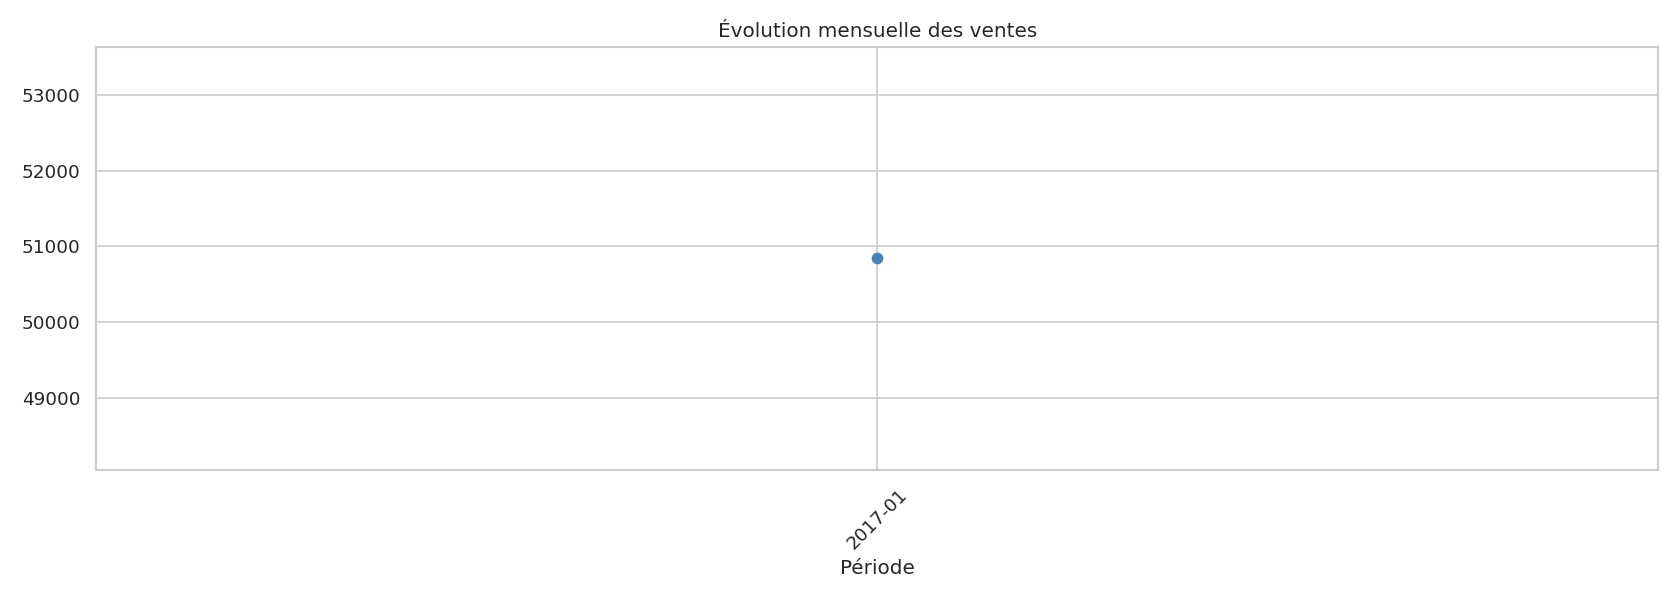
\includegraphics[width=\textwidth]{projet2/graphiques/04_evolution_ventes.png}

    \column{0.5\textwidth}
    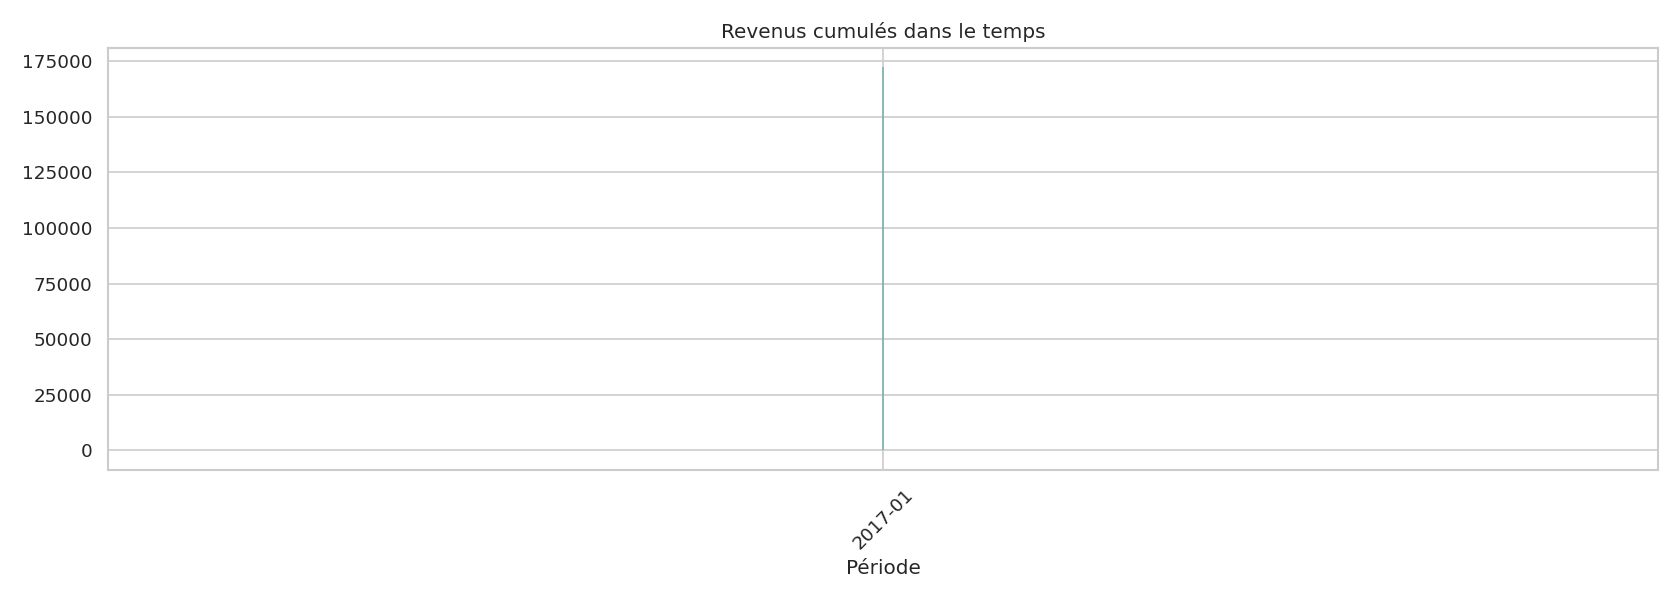
\includegraphics[width=\textwidth]{projet2/graphiques/06_revenu_cumule.png}
  \end{columns}

  \vspace{0.2cm}
  Les revenus cumulés croissent régulièrement sur la période analysée,
  confirmant une activité commerciale stable.
\end{frame}

\begin{frame}{Projet 2 --- Impact des promotions et prix}
  \begin{columns}
    \column{0.5\textwidth}
    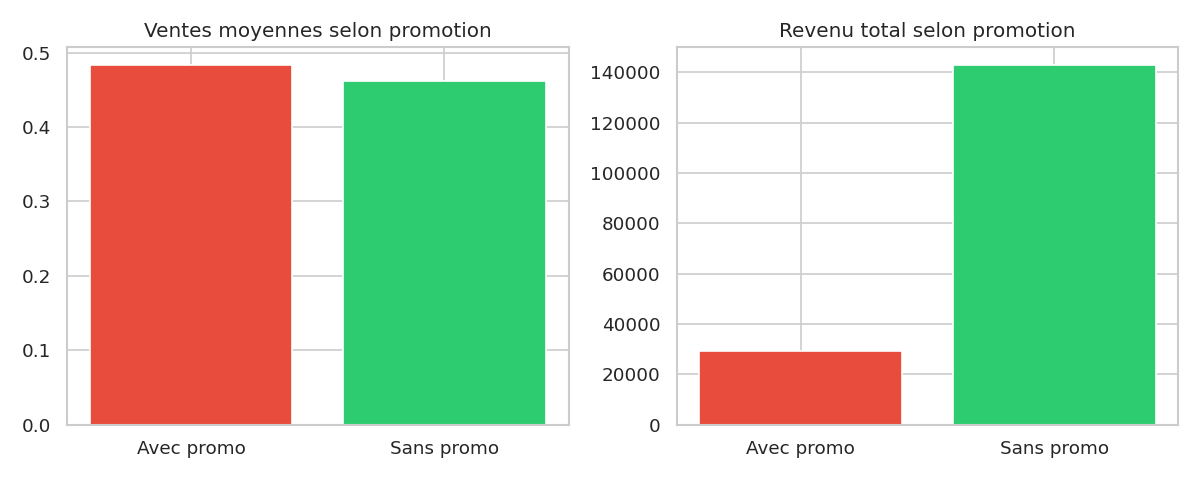
\includegraphics[width=\textwidth]{projet2/graphiques/07_impact_promotions.png}

    \column{0.5\textwidth}
    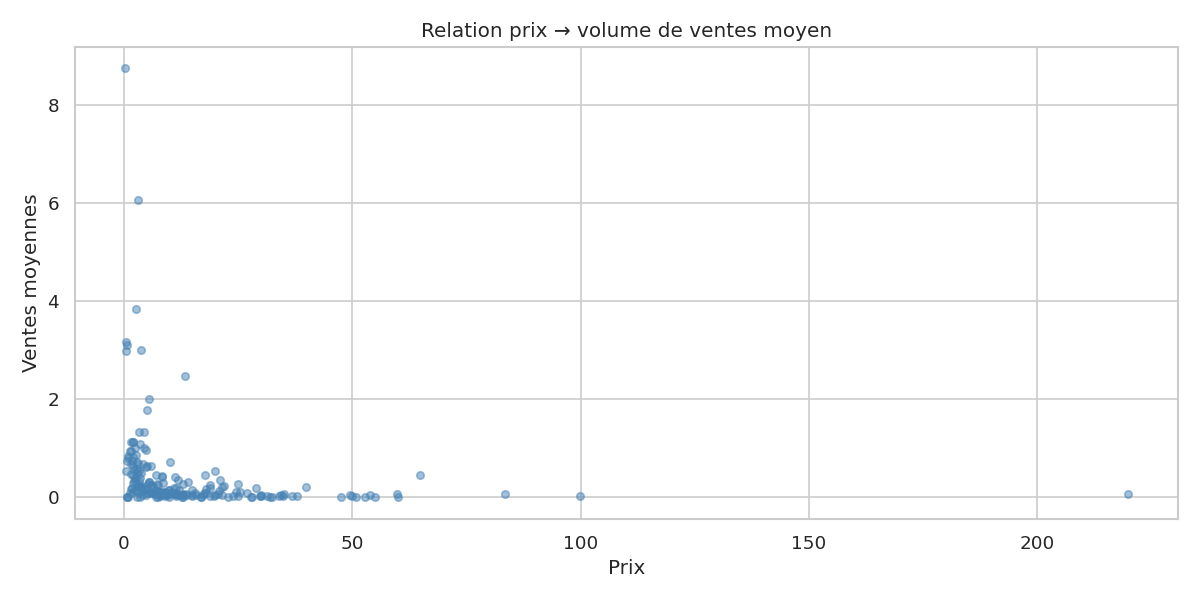
\includegraphics[width=\textwidth]{projet2/graphiques/08_prix_vs_ventes.png}
  \end{columns}

  \vspace{0.2cm}
  \begin{itemize}
    \item Les articles en promotion ont des ventes légèrement supérieures (+4.8\%)
    \item La relation prix-ventes montre une tendance négative modérée
  \end{itemize}
\end{frame}

\begin{frame}{Projet 2 --- Corrélations}
  \begin{columns}
    \column{0.5\textwidth}
    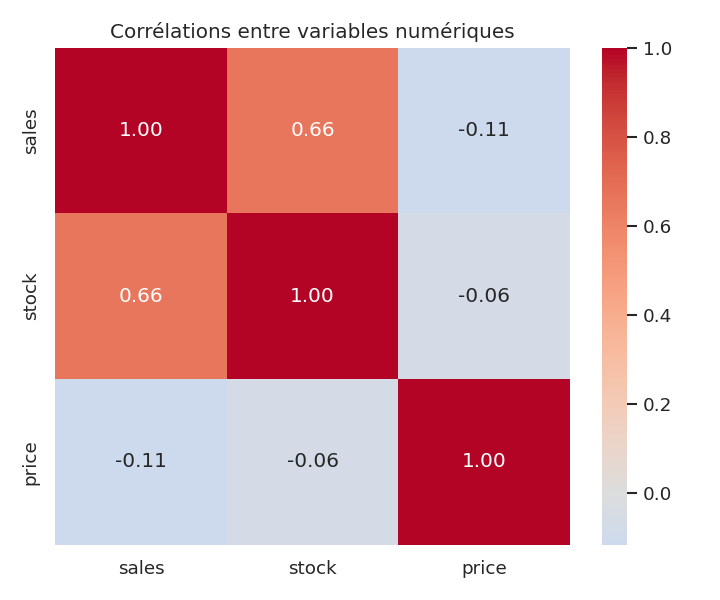
\includegraphics[width=\textwidth]{projet2/graphiques/10_correlations.png}

    \column{0.5\textwidth}
    \begin{tabular}{lc}
      \toprule
      Paire & Corr. \\
      \midrule
      sales $\leftrightarrow$ stock & \textbf{+0.45} \\
      sales $\leftrightarrow$ price & -0.11 \\
      price $\leftrightarrow$ stock & -0.11 \\
      sales $\leftrightarrow$ promo & +0.00 \\
      \bottomrule
    \end{tabular}

    \vspace{0.3cm}
    Le stock est la variable la plus corrélée aux ventes.
  \end{columns}
\end{frame}

\begin{frame}{Projet 2 --- Modélisation (Spark MLlib)}
  \begin{block}{Modèle : Régression Linéaire}
    Variables explicatives : \texttt{price}, \texttt{stock}, \texttt{en\_promotion}\\
    Variable cible : \texttt{sales}
  \end{block}

  \begin{columns}
    \column{0.5\textwidth}
    \begin{tabular}{lcc}
      \toprule
      Métrique & Valeur \\
      \midrule
      RMSE & 1.8564 \\
      MAE & 0.6802 \\
      R² & 0.1872 \\
      \bottomrule
    \end{tabular}

    \vspace{0.3cm}
    Le R² de 0.19 indique que d'autres facteurs (saisonnalité, localisation) influencent également les ventes.

    \column{0.5\textwidth}
    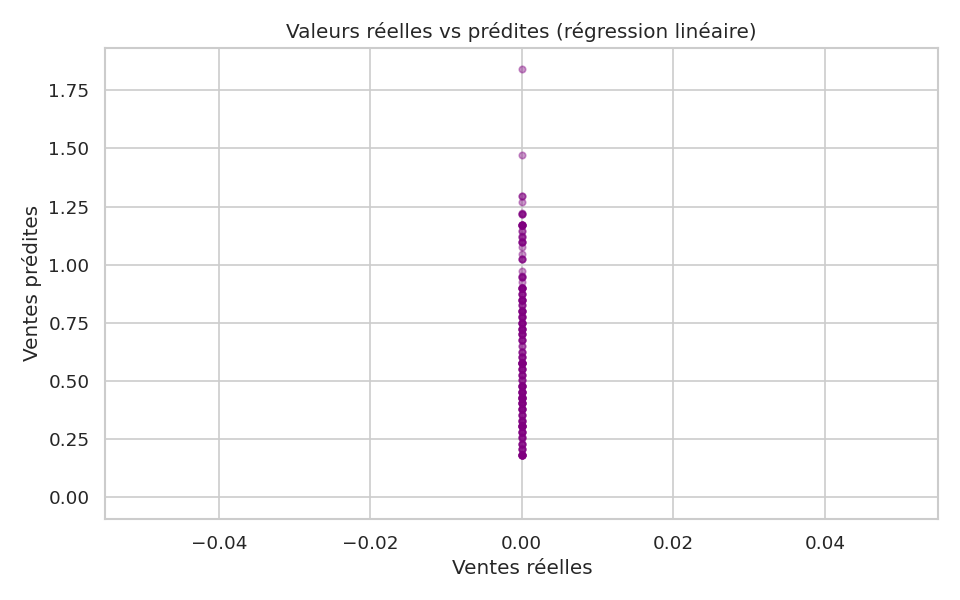
\includegraphics[width=\textwidth]{projet2/graphiques/11_reel_vs_predit.png}
  \end{columns}
\end{frame}

\begin{frame}{Projet 2 --- Recommandations}
  \begin{block}{Gestion des stocks}
    \begin{itemize}
      \item Maintenir un stock suffisant pour P0438, P0103, P0051
      \item Réapprovisionner les produits à 0 vente seulement lors de promotions
    \end{itemize}
  \end{block}

  \begin{block}{Stratégie de promotion}
    \begin{itemize}
      \item Cibler les promotions sur les produits à fort potentiel
      \item Planifier en période de faible activité saisonnière
    \end{itemize}
  \end{block}

  \begin{block}{Politique de prix}
    \begin{itemize}
      \item Produits d'entrée de gamme (bas prix) pour maximiser le volume
      \item Produits premium pour maximiser le revenu unitaire
    \end{itemize}
  \end{block}
\end{frame}

% ==========================================
\section{Conclusion}
% ==========================================

\begin{frame}{Conclusion}
  \begin{columns}
    \column{0.5\textwidth}
    \textbf{Projet 1}
    \begin{itemize}
      \item 123 répondants analysés
      \item Données nettoyées à 0 NaN
      \item 20 visualisations produites
      \item 2 segments identifiés
      \item Recommandations produit, prix et approvisionnement
    \end{itemize}

    \column{0.5\textwidth}
    \textbf{Projet 2}
    \begin{itemize}
      \item 109 442 lignes traitées avec Spark
      \item 0 NaN dans le dataset final
      \item 11 visualisations produites
      \item Modèle MLlib (R² = 0.19)
      \item Recommandations stocks, promos, prix
    \end{itemize}
  \end{columns}

  \vspace{0.5cm}
  \begin{center}
    \textbf{Code source disponible sur GitHub :}\\
    \texttt{https://github.com/Arnel7/projet-Infrastructure-Big-data}
  \end{center}
\end{frame}

\end{document}
